\documentclass{config}
\usepackage[T1]{fontenc}
\usepackage[utf8]{inputenc}
\usepackage{graphicx}
\usepackage{color}
\usepackage{siunitx}
\usepackage{listings}
\usepackage{wrapfig}
\usepackage{subcaption}
\usepackage{float}
\usepackage[toc,page]{appendix} 
\usepackage{amsmath}
\usepackage{bigints}
\usepackage{multicol}
\newcommand\x{\XSolid}

\usepackage[labelfont=sc]{caption}

%\title{}

\begin{document}

%\maketitle

I’m studying the velocity profile in one artery of approximately 13 millimeters of diameter and 7 cm of length and my probleme is that I don’t have enough points in the cross-section of the artery to obtain a physical velocity profile. I have attached figures to explain the problem. \\

Figure \ref{unzoom} (left) shows the magnitude of velocity that I obtain in the AP/IS plane at time 5/20. Figure \ref{unzoom} (right) is the same thing but on Arterys. I marked out the zone of interest in red . I feel like on Arterys there is more detail (i.e more points) that are not encoded on the velocity file that I have.

\begin{figure}[H]
\begin{minipage}{.48\textwidth}
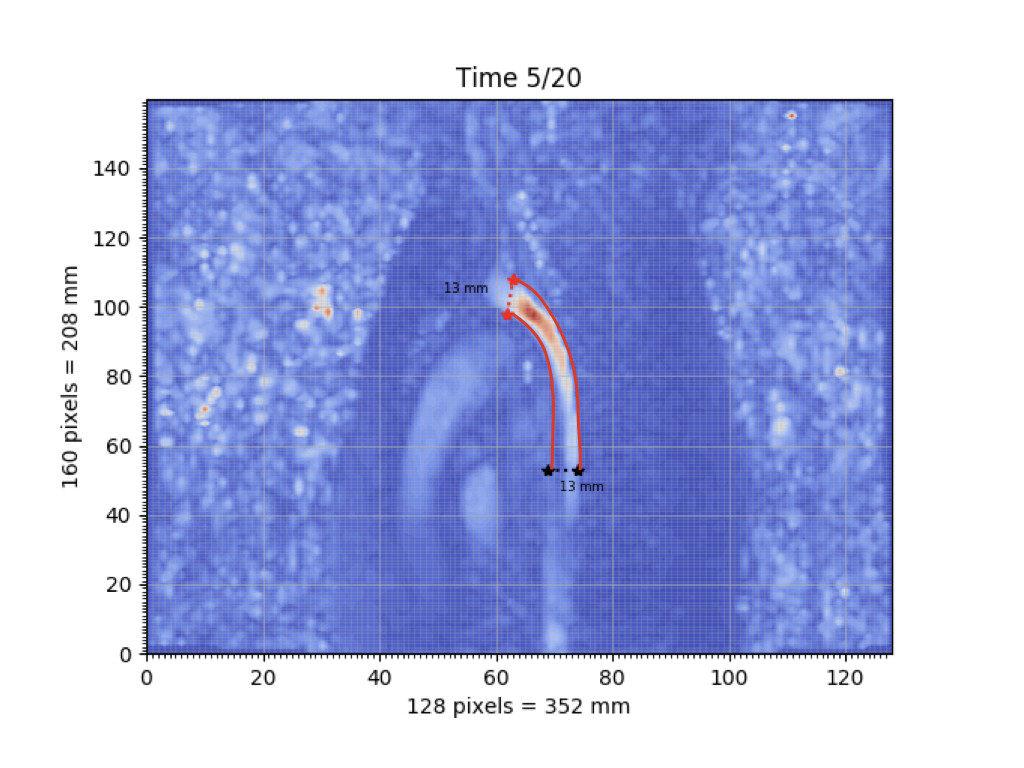
\includegraphics[scale=0.28]{Figures001.png}
\end{minipage} \hfill
\begin{minipage}{.48\textwidth}
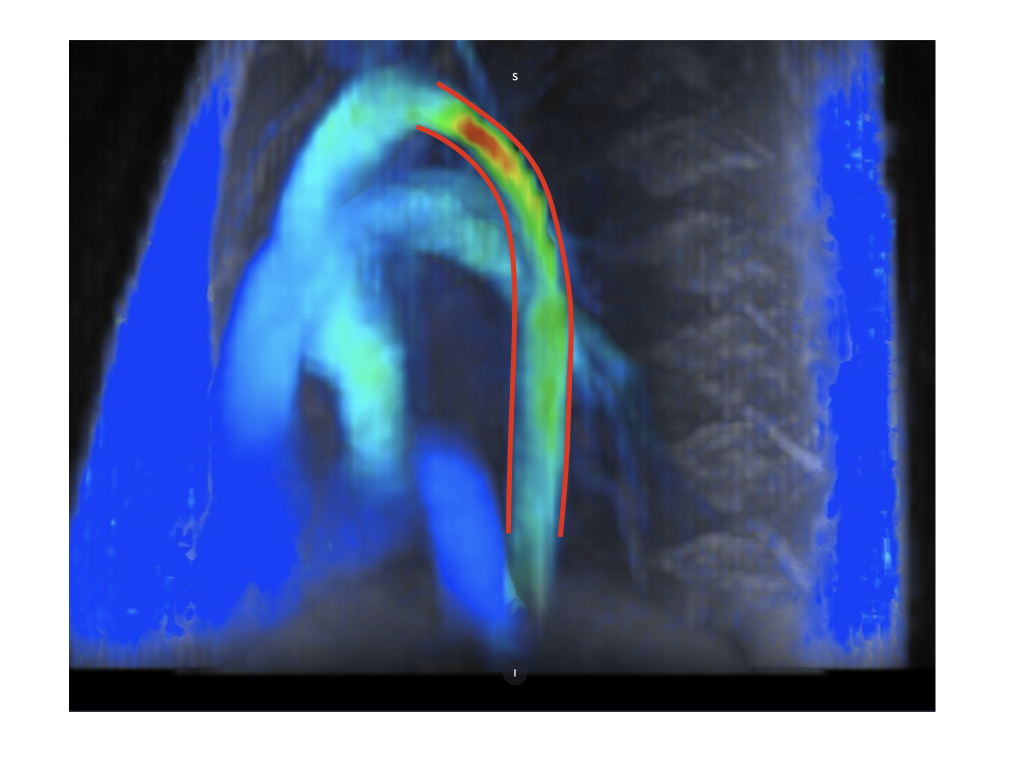
\includegraphics[scale=0.23]{Figures002.png}
\end{minipage}
\caption{Left : magnitude of velocity at time 5/20. Right : screenshot from Arterys at time 5/20 in the same plane.}
\label{unzoom}
\end{figure}

Figure \ref{zoom} is a zoom of figure \ref{unzoom} around the zone of interest. The grid corresponds to the pixels which means that at each point of the grid I have access to the velocity. As you can see on this figure, in the x-direction I only have 5 pixels for 13 mm, which seems not enough to access a physical velocity profile.

\begin{figure}[H]
\centering
\includegraphics[scale=0.67]{test2.png}
\caption{Zoom on the zone of interest highlighting the lack of pixels in one direction.}
\label{zoom}
\end{figure}


\end{document}